\documentclass[12pt]{article}

\usepackage{a4wide}
\usepackage[utf8]{inputenc}

\usepackage{amsmath}
\usepackage{graphicx}

\usepackage[osf,sc]{mathpazo}

%\pagestyle{empty}

\begin{document}

\section*{Histogram Equalization}

\noindent
Today's exercise is focused on the implementation of a histogram equalization.
\newline
\newline
\noindent
Sometimes, we acquire an image, which distribution of brightness values is quite narrow
(see example image in Fig. \ref{fig:histogram_app}).
In such image, it is hard to see details due to low contranst.
There are many techniques to achieve better contrast. In this exercise, we will cover
a simple technique.
\newline
\newline
\noindent
First, a histogram for an image has to be computed. Histogram states how many pixels in an image
have a particular value $i$. In our images, $i \in ( 0, L ]$, where $L$ stands for number of
brightness levels in the image. In our case, it is 256. A histogram value
for a value $i$ is %denoted by $n_i$.

\begin{equation} \label{eq:histogram}
    p(i) = n_i \, .
\end{equation}

\noindent
Second, we need to know the cumulative distribution function that corresponds to $p$

\begin{equation} \label{eq:cdf}
    cdf(i) = \sum\limits_{j=0}^{i} n_j \, .
\end{equation}

\noindent
Finally, we can compute the new value of brightness according to the following formula
\begin{equation}
    h(v) = \text{round} \left( \frac{cdf(v) - cdf_{\min}}{ \left( \text{width} \times \text{height} \right) - cdf_{min} } \times \left(L - 1\right) \right) \, ,
\end{equation}
where $v$ is the old brightness value, $cdf_{\min}$ is the least non-zero value of cumulative distribution function, and $h(v)$
is the the new brightness value.
\newline
\newline
\noindent
To speed up the process, you can construct a simple look-up table (LUT) of $L$ entries. You compute all the new values
in LUT and then simply go though the image brightness values and pick up the values from LUT and store them in a new image.

\newpage
\section*{Expected Output}

\begin{figure}[h]
    \centering
    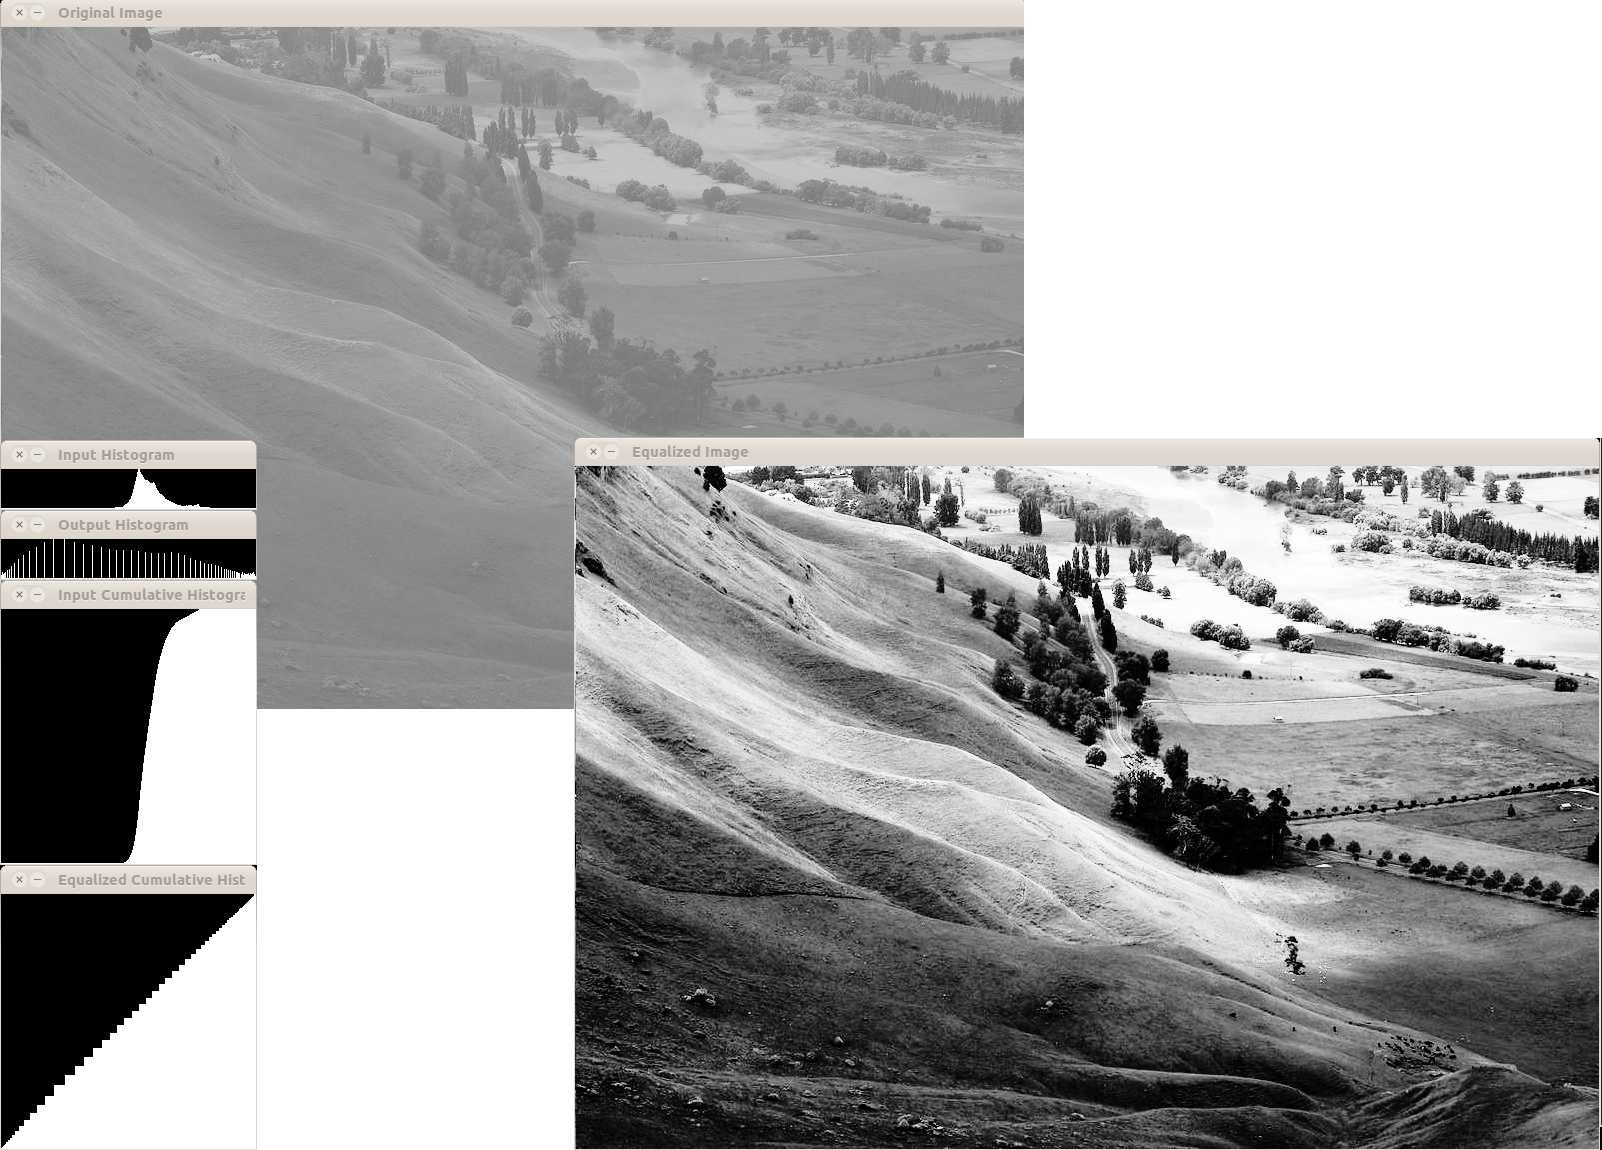
\includegraphics[width=1.0\textwidth]{hist_eq}
    \caption{An example of a histogram application. Notice the input and output histograms and cumulative distribution functions.}
    \label{fig:histogram_app}
\end{figure}

\end{document}

